\documentclass[11pt]{article}
\usepackage[utf8]{inputenc}
\usepackage[T1]{fontenc}
\usepackage{graphicx}
\usepackage{grffile}
\usepackage{longtable}
\usepackage{wrapfig}
\usepackage{rotating}
\usepackage[normalem]{ulem}
\usepackage{amsmath}
\usepackage{textcomp}
\usepackage{amssymb}
\usepackage{capt-of}
\usepackage{hyperref}
\usepackage{minted}
\usepackage{float}
\usepackage{advdate}
\usepackage[super]{nth}
\def\code#1{\texttt{#1}}
\usepackage{dirtytalk}
\usepackage{CJKutf8}
\author{Student: Mark DiValerio (mad2799) \\ Professor: Mohit Tiwari \\ TA: Austin Harris \\ Department of Electrical \& Computer Engineering \\ The University of Texas at Austin}
\date{\AdvanceDate[-1]\today}
\title{EEw382N Security Laboratory 5 Report}
\begin{document}

\maketitle
\section{Part 1 - Scanning the Internet}
\label{sec:question-1}

In this part of the lab, I scanned the internet on port 80 to see what I could find. Using an AWS EC2 c5.12xlarge instance with 12 Gbps network to alleviate the bandwidth bottleneck, I ran the zmap command:\newline\newline\code{sudo zmap –-bandwidth=100M –-target\textminus port=80 -–output-file=results\textunderscore port80.csv -b blacklist.txt -r 250 -t 10800}\newline

You can see the terminal output from the command in the screenshot below in Figure 1. After three hours, the\newline \code{part1/aws-large-results/zmap-large-ips-port80.csv} contained over 2.5 million IP addresses. I then grouped the IPs by network as you can see in the referenced file (submitted with this report) in\newline \code{part1/aws-large-results/raw-ip-grouping-port80.csv}. A statistical analysis of the network is represented in Figure 2.

\begin{figure}[H]
\centering
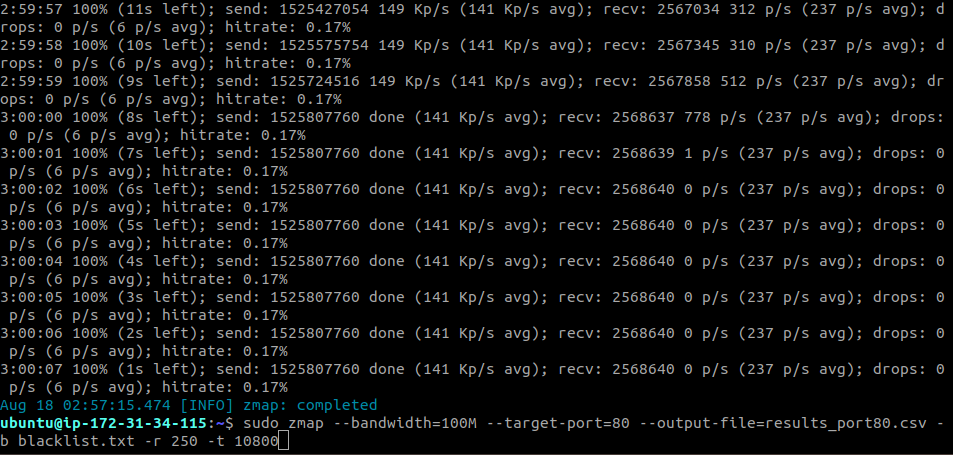
\includegraphics[width=1\textwidth]{zmap_port80.png}
\caption{\code{zmap} Terminal Output}
\end{figure}

\begin{figure}[H]
\centering
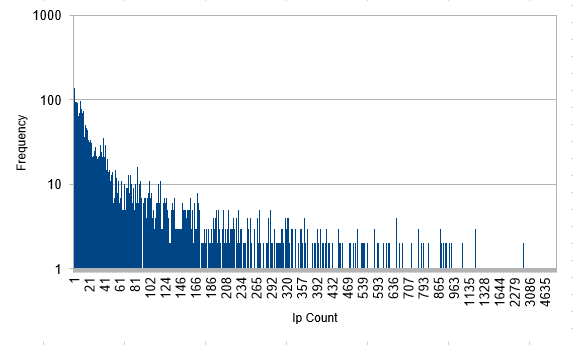
\includegraphics[width=1\textwidth]{Network IP Scan Frequency.png}
\caption{The Number of IPs a Network has and their Frequency of Occurrence}
\end{figure}


After that, I performed a \code{whois} command on the top 20 networks that contained the most IP addresses. The \code{whois} on the first IP address (with the largest network), \code{185.244.244.114}, revealed that it was a representation of all IP addresses, ranging between \code{0.0.0.0 - 255.255.255.255} for any unallocated IP. You can see the rest of my \code{whois} results in\newline \code{part1/aws-large-results/top-20-whois.txt}. They are primarily internet providers, Cloud, or Web Service companies such as Amazon, Google, and Akamai.

Once I had enough IP addresses, I wrote code to call \code{whois} and to test if the address was pingable. Of the 8,596 IP Addresses I was able to test, about 70 percent were pingable as shown in Figure 3 below. Further detail about the owner of the addresses can be seen in\newline \code{part1/aws-large-results/pingable-and-owners.xlsx}.

\begin{figure}[H]
\centering
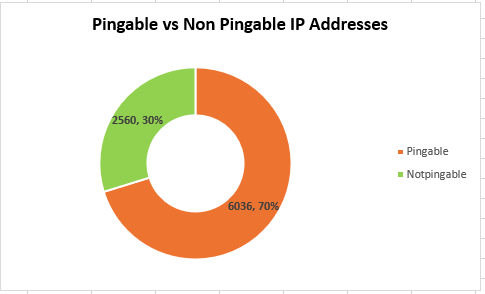
\includegraphics[width=1\textwidth]{pingable-vs-notpingable.png}
\caption{Pingable vs Not Pingable}
\end{figure}

Finally, I chose a random network to carry out a more in-depth investigation. I selected a smaller network, \code{212.200.209.8}, that contains eight IPs in total. I attempted to access and connect to each one on port 22, 80, and port 443. Of the eight IP addresses, only three of which I was able to connect via port 22 and port 80, while port 443 the connection did not time out, but it was refused. A summary of these results are represented in Figure 4. My single attempt to SSH into port 22 or visit the websites (listed from the \code{whois} command) met with a password authentication block* and a page not loading, respectively for the ports (*Did not attempt to access or break in). My investigation showed that the IP Address belonged to  Media Art Computers and the network I selected is described as the "Telekom Srbija Internet Backbone Network". You can see my whois results in the screenshot in Figure 4 below.


\begin{figure}[H]
\centering
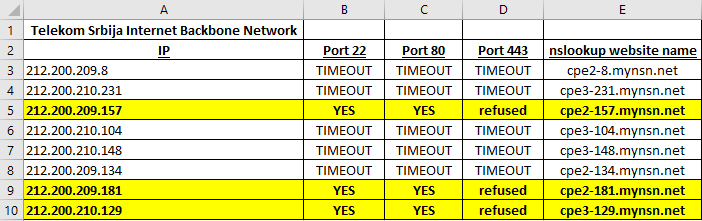
\includegraphics[width=1\textwidth]{random_network_analysis.png}
\caption{Random Network \code{212.200.209.8} Analysis}
\end{figure}


\section{Part 2 - Packet Visibility: BRO, VPN, TOR}
\label{sec:question-2}

In Part 2 of this lab, I recorded accessing ten websites, ten times each using three different connection methods for a total of 300 captured pcap files: “BRO” for using a  regular (Firefox) browser under normal connections, “VPN” for regular browser while on a VPN connection, and “TOR” for using a Tor browser on a normal connection (not VPN). During each access I performed a \code{CTRL+Shift+R} to hard-refresh so cached static content would not vary my network packets (as I would load all the cached files again) and this report's statistics. You can see all 300 pcap files in \code{part2/} directory submitted with this lab.

A statistical analysis was performed on the ten websites where average packet size and packets sent count were graphed. The data was extracted using \code{tcpdump} and the Wireshark application (Statistic/Packet Lengths menu). These results are located in the \code{part2/all\textunderscore stats} file location, each site's analysis is saved as an excel file. A sample of these results for the cat website is represented in Figure 5 and 6.

\begin{figure}[H]
\begin{minipage}[t]{0.48\textwidth}
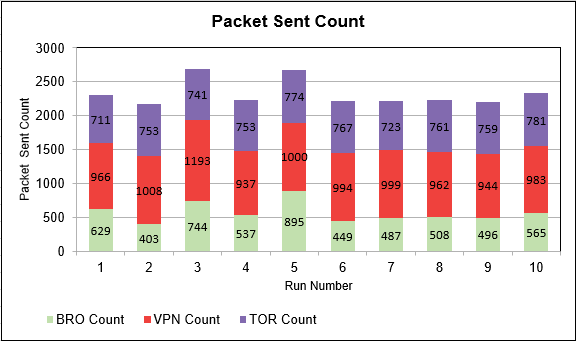
\includegraphics[width=\linewidth,keepaspectratio=true]{cat_analysis_graph_packet_sent_count.png}
\caption{Packet Sent Count - Cat}
\end{minipage}
\hspace*{\fill}
\begin{minipage}[t]{0.48\textwidth}
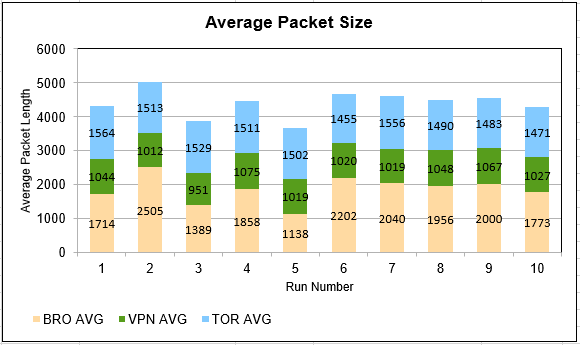
\includegraphics[width=\linewidth,keepaspectratio=true]{cat_analysis_graph_average_packet_size.png}
\caption{Average Packet Size - Cat}
\end{minipage}
\end{figure}

One interesting thing I discovered when evaluating the recordings was that VPN packets have a maximum length of 1514 bytes. This is the maximum length of a single packet but packets are normally strung together. Because I was using a VPN, only individual packets are evaluated.

For VPN, I was able to identify the destination location easily by following the TCP (utexas) trace, however the same method did not work for the TOR packets as you can see in the highlighted sections in Figure 7 below.

\begin{figure}[H]
\centering
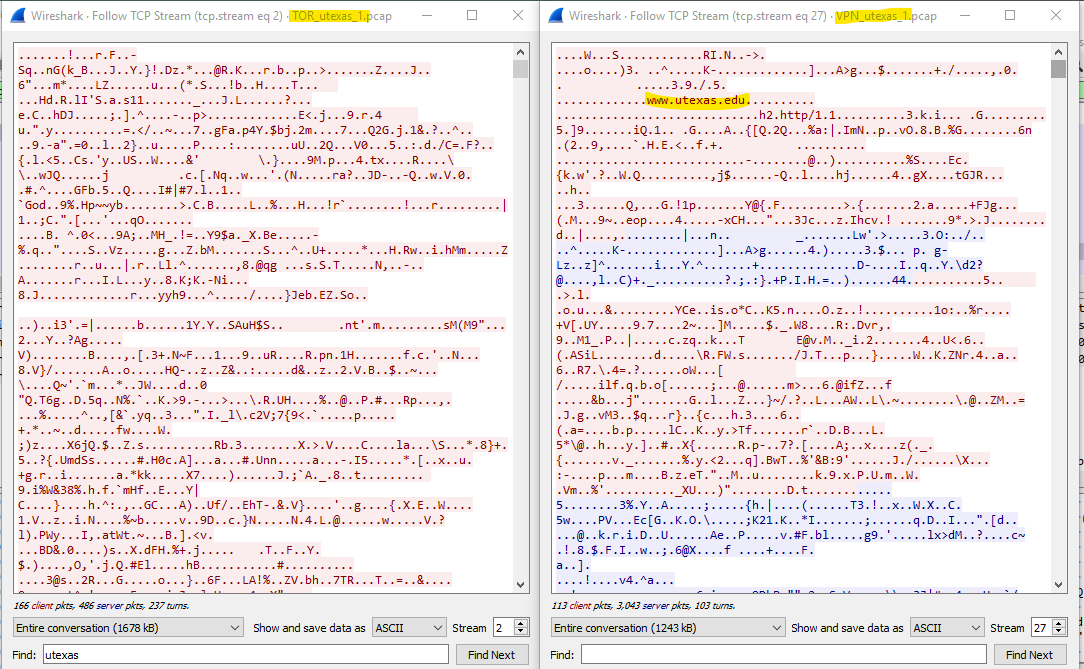
\includegraphics[width=1\textwidth]{vpn_vs_tor.png}
\caption{Left is TOR, Right is VPN}
\end{figure}



\section{Conclusion}
\label{sec:conclusion}
In conclusion, this lab was interesting to investigate and scan the vast IP addresses around the world, learning the network tools, and the differences between TOR and VPN. Creating statistical analyses of each gave me insight into how the packets are made and what they look like. My only feedback for this lab was the time constraint. Scanning enough IP addresses for a report and performing analysis on 300 pcap files made each minute precious, although I understand since it is the summer semester and we only have so much time.


\bibliography{bibliography}
\bibliographystyle{ieeetr}
\end{document}
